% !TEX root = ../../thesis.tex

\section{Motivation for Formal Syntax Descriptions}

To be able to run tests automated on every kind of KeTop, there is a need to modify test scripts depending on the given environment. That is why an extended Robot Framework language was needed. The Extended Backus-Naur Form (EBNF) was chosen for this, to make this new language easily extendable and deterministic to implement if adopted by other developers.

In practice, in the field of computer science, it is clear that a precise description of a language is the most important foundation. It is therefore essential that applications, communication protocols or programs function according to clear syntactic rules so that they are always interpreted in the same way by humans and machines. Natural language provides many different ways of describing something. There are ambiguities in language, and these can lead to errors in interpretation. These findings are not new. They have been known for a long time. Nevertheless, there is still no common standard that everyone adheres to, especially when languages have been implemented independently by different developers~\cite[p.~V]{ISO/IEC149771996InformationBNF}.

Syntactic metalanguages exist to solve this problem. The goal of a metalanguage is to describe another language. This means there is a difference between the language that is described and the language used to describe it.

In programming, a metalanguage is a language used to describe the syntax and structure of another language, called the object language. For example, BNF and EBNF are metalanguages used to define programming languages such as ALGOL. The structure of sentences and expressions in a metalanguage can be defined using a so-called metasyntax. For example, one could indicate that the word ``noun'' can itself function as a noun in a sentence by writing: ``noun'' is a \texttt{<noun>}~\cite{WikipediaMetalanguage}.


\section{The Backus-Naur Form (BNF)}

One of the most important metalanguages for programming has been BNF (the so-called Backus-Naur Form). BNF started with ALGOL 60 in 1960. ALGOL 60 needed a clear, formal way to describe its syntax. John Backus and Peter Naur therefore created BNF. It made it possible to define language rules precisely. This was the first time syntax was described formally. The history of ALGOL 60 is crucial because it gave BNF its first real use. BNF became the foundation for defining many programming languages. It is still essential in compilers and language design today~\cite[ p.~3]{Mossenbock2025}.

As BNF was first used for ALGOL 60 and became the model for many later languages, over time, people added changes or extensions, which created some confusion. Despite this, BNF showed the importance of clear, formal syntax.

Therefore, Extended BNF was later developed from BNF and included the most common extensions. The large amount of variants motivated the standardization effort that resulted in the standard named \emph{ISO/IEC~14977} by the International Organization for Standardization~(ISO)~\cite[p.~V]{ISO/IEC149771996InformationBNF}.

\section{The Evolution to Extended BNF (EBNF)}

For early programming languages such as ALGOL 60, BNF was adequate. However, the increased complexity of modern languages required a more systematic notation to describe their syntax effectively.

Therefore, the so-called Extended Backus-Naur Form (EBNF) was introduced. The inventor of Extended BNF - EBNF, is Niklaus Wirth, a Swiss computer scientist. EBNF is based on BNF but it adds more elements.

\begin{quote}
``One cannot fail to notice the lack of "common denominators."''~\cite{Wirth1977WhatDefinitions}
\end{quote}

Niklaus Wirth stated this in his first article in the journal ``Communications of the ACM'' in 1977 about EBNF.

He explained that there is a lack of common standards or unified fundamental principles across different language definitions and notational forms. Each language definition tends to use slightly different variants of the Backus-Naur form based notation. There is no generally accepted standard, and the differences are often small but unnecessarily varied. He stated that a more uniform notation would improve scientific work and comparison. EBNF is his solution for this problem. 

As mentioned EBNF is clearly based on BNF, but it adds more elements. EBNF can define exact numbers of elements, describe exceptions, add comments, use flexible rule names, and allow extensions. This makes grammar definitions shorter and it is easier to read them. But EBNF also has restrictions. It can only handle languages with elements in order and is not able to describe very complex grammar~\cite[pp.~VII-VIII]{ISO/IEC149771996InformationBNF}.

The main disadvantage of BNF according to ISO/IEC~14977 was:

\begin{quote}
``Backus-Naur Form (used in ALGOL 60) has problems if the metasymbols \texttt{< > ::=} occur in the language being defined. Some common forms of construction (e.g.\ comments) cannot be expressed naturally; other constructions (e.g.\ repetition) are long winded.''~\cite[p.~VII]{ISO/IEC149771996InformationBNF}
\end{quote}


The added advantages, but also the limitations of EBNF, will be discussed in more detail in later sections and chapters.

\section{Wirth's Approach to Syntax Definition}

Having established the historical need for a unified standard in the previous section, it is now necessary to examine the concrete syntactic rules proposed by Niklaus Wirth in 1977. In his article published in the journal Communications of the ACM (CACM), Wirth addressed the existing problems of syntactic notation directly. His contribution marked an important step in the formal development of language definitions.

Wirth did not intend to introduce a completely new theoretical concept. Instead, his objective was to improve the existing Backus-Naur Form in a systematic way. BNF had already proven to be useful. However, it contained ambiguities and practical limitations.

The notation presented in his article was therefore designed to be more practical and clearer in structure. It focused on improving readability and standardization rather than expanding theoretical expressive power. The goal was not innovation for its own sake. The goal was clarity, consistency, and easier application in real technical environments.

Wirth listed the following properties to extend BNF~\cite{Wirth1977WhatDefinitions}:

\begin{enumerate}
    \item The notation clearly separates meta symbols, terminal symbols, and nonterminal symbols. \\
    Example: \texttt{syntax = "production".} \\
    Here, \texttt{syntax} is a nonterminal symbol. \texttt{"production"} is a terminal symbol. The equals sign and the dot are structural meta symbols.
    
    \item Symbols used for structure can also be used as normal language symbols. This avoids artificial restrictions. \\
    Example: If quotation marks are used as meta symbols, they can still appear inside text if written twice, like \texttt{""} in many programming languages.
    
    \item The notation contains a simple way to express repetition. This reduces the need for recursion in simple cases.
    
    \item The notation avoids explicit representation of the empty string, such as by using \texttt{<empty>} or $\varepsilon$.
    
    \item The notation is based on the \gls{ascii} character set. This makes it easy to use in most technical environments.
\end{enumerate}

In his article, he showed the power of EBNF by defining its own syntax as an example (see Figure~\ref{fig:defebnf}):

\begin{quote}
``This meta language can therefore conveniently be used to define its own syntax, which may serve here as an example of its use. The word identifier is used to denote nonterminal symbol, and literal stands for terminal symbol. For brevity, identifier and character are not defined in further detail.''\cite{Wirth1977WhatDefinitions}
\end{quote}

\begin{figure}[h]
    \centering
    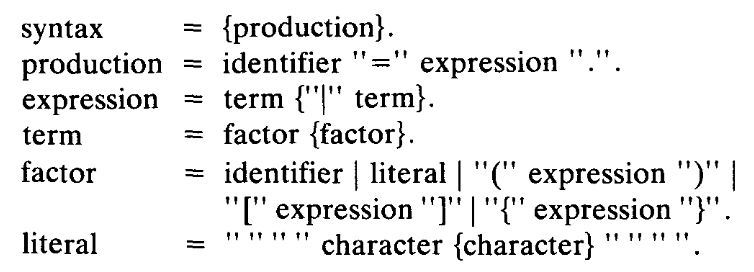
\includegraphics[width=0.75\linewidth]{pics/Definition_of_EBNF_in_EBNF.png}
    \caption{Definition of EBNF in EBNF in ``What Can We Do about the Unnecessary Diversity of Notation for Syntactic Definitions?'' from N. Wirth~\cite{Wirth1977WhatDefinitions}}
    \label{fig:defebnf}
\end{figure}


\section{Core Syntactic Extensions}

The following overview focuses in more detail on the differences between BNF and Extended Backus-Naur Form (EBNF) as described in Concepts of Programming Languages by Robert W. Sebesta~\cite[pp.~149-151]{SebestaConceptsEdition}.

It is worth noting that these extensions do not add to the descriptive capabilities of BNF. Their purpose is simply to make formal grammars easier to read and write. BNF is theoretically sufficient for describing context-free languages, but EBNF provides a more concise notation for complex structures.

\subsection{Core Syntactic Extensions in EBNF in detail}

Sebesta identifies three primary extensions common to most versions of EBNF:

\begin{itemize}
    \item \textbf{Optionality} (\texttt{[...]}): \\
    Brackets are used to denote a part of a right-hand side (RHS) that may occur once or not at all. \\
    Example: \texttt{[meow]} means meow or empty.
    
    \item \textbf{Repetition} (\texttt{\{...\}}): \\
    Braces indicate that the enclosed part can be repeated any number of times, including zero. This replaces the need for recursion when describing simple lists. \\
    Example: \texttt{\{chirp\}} can be empty, chirp, chirpchirp, chirpchirpchirp, and so on. \\
    Example for the usage for lists: \texttt{list = <item> \{<item>\}}, which represents a list of one or more items.
    
    \item \textbf{Multiple-Choice Options} (\texttt{(...|...)}): \\
    A set of alternatives can be written in parentheses, with the vertical bar (i.e., the OR operator \texttt{|}) used to separate the possible choices. \\
    Example: \texttt{(pancake | waffle)} represents either pancake or waffle.
\end{itemize}

In this notation, brackets, braces, and parentheses serve as metasymbols rather than terminal symbols of the language being described~\cite[pp.~149-151]{SebestaConceptsEdition}.

\subsection{Further Syntactic Extensions in EBNF based on ISO/IEC 14977}

However, there are more differences between BNF and EBNF in the ISO/IEC 14977 definition:~\cite[p.~VII]{ISO/IEC149771996InformationBNF}

\begin{itemize}
    \item \textbf{Defining an explicit number of items:} In some cases it is needed to describe, that e.g., a field must have an exact length. In BNF, this is difficult. Often, the programmer has explained it then informally in English. Now EBNF solves this by allowing an integer followed by a repetition-symbol (\texttt{*}). With this solution, the programmer can specify the exact number of items. This makes rules much shorter.
    
    \item \textbf{Exceptions:} Sometimes it would be easier to define a rule by specifying what is not allowed. But BNF cannot easily say ``any character except a quote''. EBNF has a solution for that. EBNF uses an except-symbol (\texttt{-}) to define rules by exclusion. This makes definitions shorter and easier. Therefore, for example, a programmer can define a group of symbols and then subtract specific exceptional cases, such as ``any character except a quote''.
    
    \item \textbf{Formal comments:} Comments are an important feature, that BNF is not offering. EBNF provides a formal way to add comments using \texttt{(*} and \texttt{*)}. And these notes do not change the machine's logic.
    
    \item \textbf{Flexible names:} In BNF, names for categories often need brackets. EBNF uses an explicit comma (\texttt{,}) as a so-called concatenate symbol to link parts of a rule. This removes the restriction that category names or meta-identifiers must be single words or enclosed in brackets, allowing for more flexible naming. It also ensures that the layout of the syntax like spaces or line breaks has no effect on the defined language.
    
    \item \textbf{Extensions:} Programmers can add their own features to EBNF. These are called ``special sequences'' and are placed between question marks (\texttt{?}). This makes the start and end of any extension very easy to find. Extensions were used several times in earlier versions of the solution presented in this thesis, but were eliminated in the final version because there was no longer a need for them.
\end{itemize}

\subsection{Comparative Notation BNF and EBNF}

While classical BNF is theoretically sufficient for describing any context-free language, it is often complicated and repetitive in practice. The main cause therefore is, that it relies, as described in the previous chapter, exclusively on recursion to express lists and optional elements. In the following illustration one can see the advantage of EBNF introducing specialized meta symbols, such as braces, brackets, and parentheses~\cite[p.~153]{SebestaConceptsEdition}.

\begin{figure}[h]
    \centering
    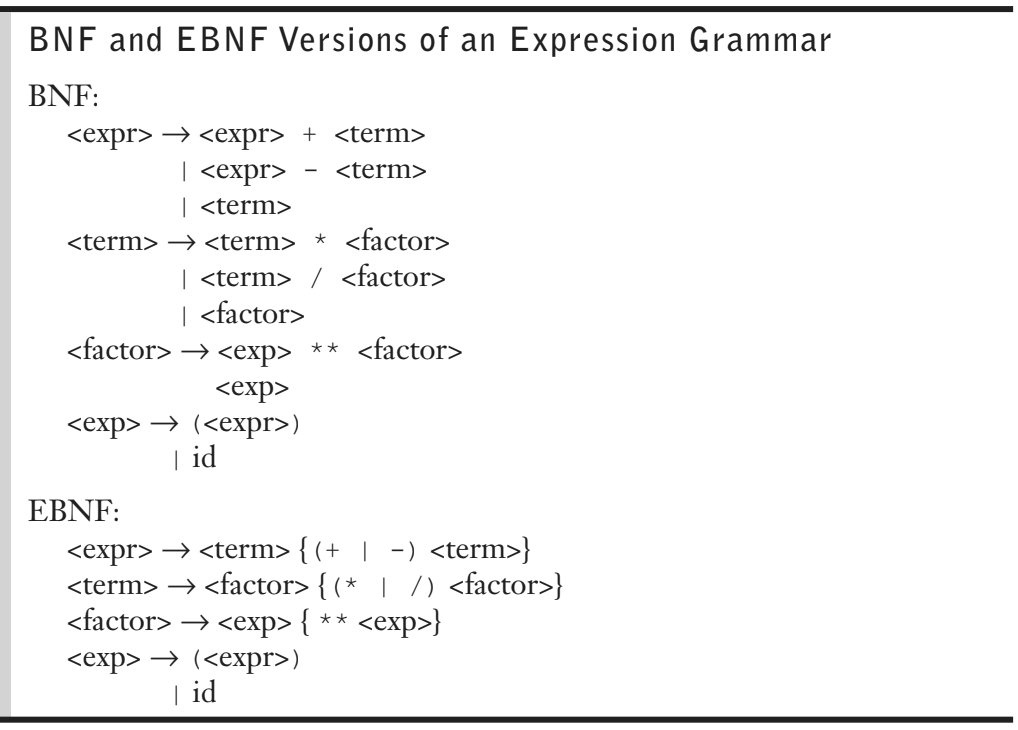
\includegraphics[width=0.75\linewidth]{pics/BNFANDEBNF.png}
    \caption{Comparison between BNF and EBNF by Sebesta~\cite[p.~153]{SebestaConceptsEdition}}
    \label{fig:bnfvsebnf}
\end{figure}


As demonstrated in the example in Figure~\ref{fig:bnfvsebnf}, the structural differences lead to a significant reduction in the number of rules required:

\begin{itemize}
    \item \textbf{Repetition via Braces in this example:} In the BNF version of the expression grammar, an \texttt{<expr>} must be defined recursively to handle a sequence of additions or subtractions. EBNF replaces this recursion with braces \texttt{\{...\}}, which denote that the enclosed part can be repeated indefinitely or left out entirely.
    \item \textbf{Multiple-Choice Options in this Example:} The example uses parentheses \texttt{(...)} combined with the OR operator \texttt{|} to group choices. This for example allows the EBNF version to handle both addition and subtraction in a single line. In BNF it requires a more complex approach.
\end{itemize}

\subsection{Modern Variations and Standardization}

While an official standard exists (ISO/IEC~14977:1996), it is rarely used in practice. There have several variations of EBNF emerged in recent years, which deviate from the standardized syntax, such as using a colon instead of an equal sign or a dot instead of a semicolon. Also the project described in this thesis partially deviates from ISO standards due to using the EBNF dialect of the Lark Python library. 

\section{ISO/IEC 14977 Standards for Assembler Logic}

While the previous chapters describe the advantages of EBNF in terms of readability and compactness, the ISO definition has an additional function. The ISO standard ISO/IEC 14977 also defines strict technical rules.

These are very important for error-free processing by an automated tool such as a script assembler, as they ensure that the grammar definition remains mathematically unambiguous.

\subsection{Operator Precedence}

For every EBNF grammar, the strictly defined hierarchy of meta-symbols is essential, as it prevents ambiguities in the rules.
The order of the symbols is clearly defined in the ISO standard without any leeway and is specified as follows: (the strongest is the repetition symbol. This takes precedence, followed by the exclude symbol, and so on).
\begin{enumerate}
\item Repetition symbol (*): For specifying exact numbers of repetitions.
\item Except symbol (-): For defining sets by exclusion.
\item Concatenate symbol (,): For explicitly linking consecutive elements.
\item Definition separator symbol (|): For separating alternatives.
\item Defining symbol (=): Formally assigns an expression to a nonterminal.
\item Terminator symbol (;): To clearly mark the end of a production rule.
\end{enumerate}

\cite[p.~1]{ISO/IEC149771996InformationBNF}

\subsection{Layout Neutrality Through Gap Separators}

Ideally, a script assembler should be able to process scripts regardless of their visual formatting. The ISO standard is helpful here, as it defines so-called ``gap separators'' (such as spaces, tabs, or line breaks)~\cite[pp.~5]{ISO/IEC149771996InformationBNF}. These characters have no formal meaning outside of terminal strings. This has the significant advantage of allowing for flexible grammar design without affecting the assembler's logic. Since gap separators and comments have no formal effect on the defined language, the script assembler can ignore these characters during analysis, which, for example, increases its robustness against different programming styles.

In summary, several advantages arise. The grammar definition remains mathematically consistent for automated tools. Furthermore, it is beneficial that the grammar can be made more readable and understandable for human readers through formatting and annotations.

\subsection{Syntactic Exceptions}

As mentioned earlier, the Except symbol (\texttt{-}) allows the assembler to define specific instruction sets. An example of this would be ``all characters except a semicolon.'' However, the ISO standard also imposes very clear technical limitations on this function, as otherwise paradoxes could arise:

\begin{quote}
``If a syntactic exception is permitted to be an arbitrary syntactic factor, Extended BNF could define a wider class of languages than the context-free grammars, including attempts which lead to Russell-like paradoxes... Such a license is undesirable and the form of a syntactic exception is therefore restricted to cases that can be proved to be safe.''~\cite[p.~2]{ISO/IEC149771996InformationBNF}
\end{quote}

A good explanation for the Russell Paradox, formulated by Bertrand Russell, is the so-called barber's example: In a village, the barber shaves precisely all the men who don't shave themselves, and only these men. The question of whether the barber shaves himself leads directly to a contradiction: If he shaves himself, he shouldn't, by definition; if he doesn't shave himself, he should~\cite{WikipediaBarbierParadoxon}.

This example illustrates that such self-referential definitions can lead to logical inconsistencies in formal systems.


\subsection{Alternative Representations for System Compatibility}

To guarantee that a grammar functions on different systems, the ISO standard allows the substitution of certain special characters if they are missing. For example, the characters \texttt{(:} and \texttt{:)} can replace \texttt{\{} and \texttt{\}}, or a period (\texttt{.}) can replace a semicolon at the end of a rule. This ensures that the grammar remains readable and functional on different platforms without losing its original structure~\cite[p.~5]{ISO/IEC149771996InformationBNF}.

\subsection{Special Sequences as a Formal Interface for Assembler Extensions}

Although special sequences were already described in the previous section as a general extension option, they are listed again here to specifically clarify their ``technical'' role as placeholders. In the logic of a script assembler, they serve as a standardized mechanism to mark parts of the language that cannot be defined by EBNF itself (e.g., specific character sets)~\cite[p.~VII]{ISO/IEC149771996InformationBNF}.

By enclosing them in question marks (\texttt{?...?}), the grammar remains formally valid for the assembler tool. In this work, they thus can provided the flexibility for possible future functional extensions without violating the fundamental syntactic rules of the ISO standard~\cite[p.~3]{ISO/IEC149771996InformationBNF}.


\subsection{Evaluating the Standard for our Script Assembler}

After introducing the theoretical foundations of EBNF, it is necessary to evaluate how the ISO standard was applied in the context of the script assembler. The goal of the project was not to implement a complete parser for the Robot Framework. Instead, the focus was on building a preprocessor for specific control tags such as \texttt{@OS}. For this reason, the resulting grammar is not a strict implementation of the ISO standard. It represents a pragmatic combination of formal rules and practical requirements.

A central aspect of this evaluation is the concept of layout neutrality. The ISO standard defines spaces, tabs, and line breaks as so-called gap separators. These elements have no formal meaning and can be ignored by the parser. This principle improves flexibility and readability. However, it could not be applied completely in this project. Inline spaces and tabs between control tokens are treated as insignificant and are therefore ignored. This allows test scripts to remain flexible in their formatting.

Line breaks, however, require a different treatment. Robot Framework scripts are structured line by line. This means that line breaks carry semantic meaning. They define the structure of the script. Therefore, line breaks could not be treated as layout-neutral elements. Instead, they were explicitly defined as structural tokens in the grammar. This is a necessary deviation from the ISO specification to ensure correct processing of the input.

Further deviations from the standard were made in the handling of syntactic constraints. The ISO standard introduces syntactic exceptions to define rules by exclusion. However, this mechanism can become complex and difficult to understand. In some cases, it can even lead to problematic definitions. For this reason, syntactic exceptions were not used in the assembler.

Instead, the implementation relies on regular expressions. \Gls{regex} provides a practical way to capture and process text patterns. It allows the parser to treat sections of Robot Framework code as plain content. The internal structure of these sections is not analyzed. This simplifies the grammar and reduces its complexity. As a result, the grammar becomes easier to read and maintain.